\section{Конструкторская часть}

% Кратко описать, что будет в конструкторской части

В данной части будут приведены требования к программному обеспечению, на формальном языке будут описаны алгоритмы, которые будут реализованы при разработке программного обеспечения, а также будет обоснован выбор типов и структур, которые будут использованы при разработке, и приведена общая архитектура разрабатываемой программы.

\subsection{Требования к программному обеспечению}

% Составить ТЗ, что должна делать программа

Разрабатываемое программное обеспечение должно предоставлять пользователю следующую функциональность:
\begin{itemize}
    \item добавление объекта на сцену (куб, сфера, чайник);
    \item выбор объекта сцены с помощью клавиатуры;
    \item изменение цвета выбранного объекта;
    \item изменение геометрических свойств выбранного объекта (положение в пространстве, поворот, увеличение);
    \item изменение физических свойств выбранного объекта (масса, скорость, ускорение, сила);
    \item изменение значения гравитации;
    \item перемещение и поворот камеры с помощью клавиатуры и мыши.
\end{itemize}

При этом разрабатываемая программа должна удовлетворять следующим требованиям:
\begin{itemize}
    \item программа должна генерировать кадр не менее, чем за $\frac{1}{60}$ секунды;
    \item никакие действия пользователя не должны приводить к аварийному завершению программы.
\end{itemize}

\subsection{Разработка алгоритмов}

Далее на формальном языке будут описаны алгоритмы, которые будут реализованы при разработке проргаммного обеспечения.

\subsubsection{Общий алгоритм работы программы}

Далее представлен общий алгоритм работы разрабатываемого программного обеспечения.

\begin{enumerate}
    \item Инициализировать используемые объекты (окно, камера, сцена, объекты сцены, графический интерфейс, шейдерная программа).
    \item Пока приложение запущено:
        \begin{itemize}
            \item обработать события от мыши и клавиатуры;
            \item обнаружить и разрешить коллизии;
            \item обновить местоположения объектов сцены;
            \item сгенерировать и отобразить кадр.
        \end{itemize}
    \item Освободить ресурсы.
\end{enumerate}

% \subsubsection{Алгоритм, использующий z-буфер}

\subsubsection{Алгоритм AABB}

На рисунке \ref{fig:aabb} представлена схема алгоритма AABB обнаружения коллизий.

\begin{figure}[H]
	\centering
	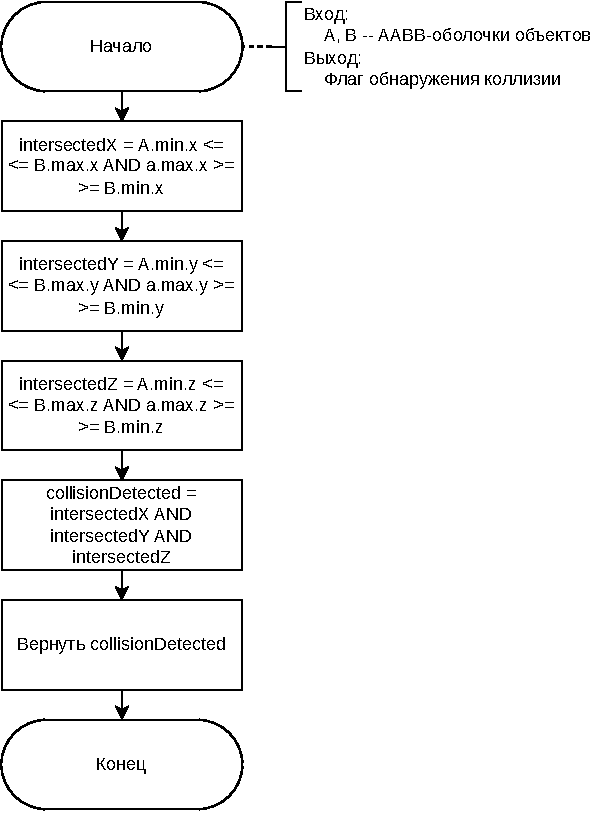
\includegraphics[scale=1]{diag/aabb.pdf}
	\caption{Алгоритм AABB обнаружения коллизий}
	\label{fig:aabb}
\end{figure}

% \subsubsection{Алгоритм GJK}

% \subsubsection{Алгоритм EPA}

\subsubsection{Модель освещения Фонга}

В модели освещения Фонга \cite{realphong, phong, rogers} учитываются три составляющих отражённого света:
\begin{enumerate}
    \item рассеянная,
    \item фоновая,
    \item зеркальная.
\end{enumerate}

\subsubsection*{Рассеянный свет}

Рассеянный свет является светом, отражаемым во всех направлениях, и его интенсивность во всех направлениях постоянна, следовательно, для его рассчёта не требуется учитывать направление взгляда камеры, но должен быть известен угол между направлением света и нормалью к поверхности объекта \cite{phong}.

\begin{figure}[H]
	\centering
	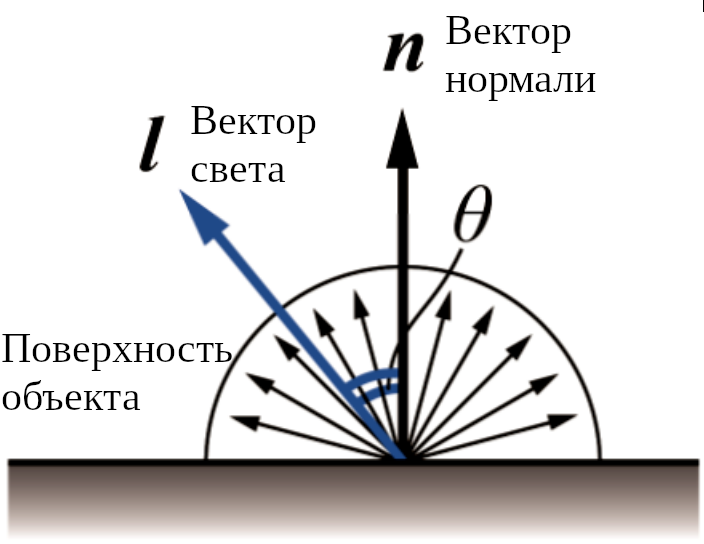
\includegraphics[width=0.56\textwidth]{img/diffuse_ru}
    \caption{Модель Фонга: Рассеянная составляющая света (Источник: \cite{phong})}
	\label{fig:diffuse}
\end{figure}

Рассеянная составляющая света, согласно \cite{phong}, рассчитывается по формуле~\ref{eq:diffuse}, приведённой ниже.

\begin{equation}
    I_d = k_d I_l \cos \theta = k_d I_l \left| \boldsymbol{n} \cdot \boldsymbol{l} \right|,
    \label{eq:diffuse}
\end{equation}
где 
\begin{itemize}
    \item $I_l$ --- интенсивность источника света,
    \item $k_d$ --- коэффициент рассеивания света,
    \item $\boldsymbol{n}$ --- вектор нормали к поверхности объекта,
    \item $\boldsymbol{l}$ --- вектор направления света,
    \item $\cos \theta$ --- угол между вектором направления света и нормалью к поверхности объекта.
\end{itemize}

\subsubsection*{Фоновое освещение}

Если учитывать только рассеяный свет при освещении объекта, будут видны абсолютно неосвещённые, чёрные грани.
В реальном мире такое встречается редко, в связи с чем, для достижения большей реалистичности, было предложено ввести минимальный уровень освещённости --- фоновое освещение, являющееся обычно результатом отражения света от других объектов сцены~\cite{phong, quakecon}.

\begin{figure}[H]
	\centering
	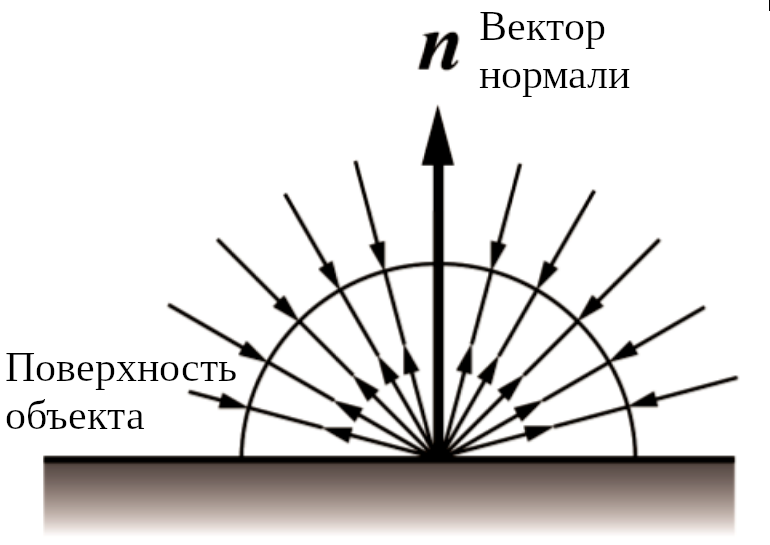
\includegraphics[width=0.6\textwidth]{img/ambient_ru}
    \caption{Модель Фонга: Фоновая составляющая света (Источник: \cite{phong})}
	\label{fig:ambient}
\end{figure}

Фоновая составляющая света, согласно \cite{phong}, рассчитывается по формуле~\ref{eq:ambient}, приведённой ниже.
\begin{equation}
    I_a = k_a I_0,
    \label{eq:ambient}
\end{equation}
где
\begin{itemize}
    \item $k_a$ --- отражательная способность объекта,
    \item $I_0$ --- интенсивность фонового освещения.
\end{itemize}

\subsubsection*{Зеркальный свет}

В реальном мире гладкие объекты отражают свет подобно зеркалу --- чем менее объект шероховатый, тем более отчётливо он отражает источник света, и виден блик.
Для достижения подобного эффекта было предложено использовать функцию косинуса и регулировать размытость границ блика с помощью возведения косинуса угла между вектором взгляда и отражённым светом в различные степени \cite{quakecon}.

\begin{figure}[H]
	\centering
	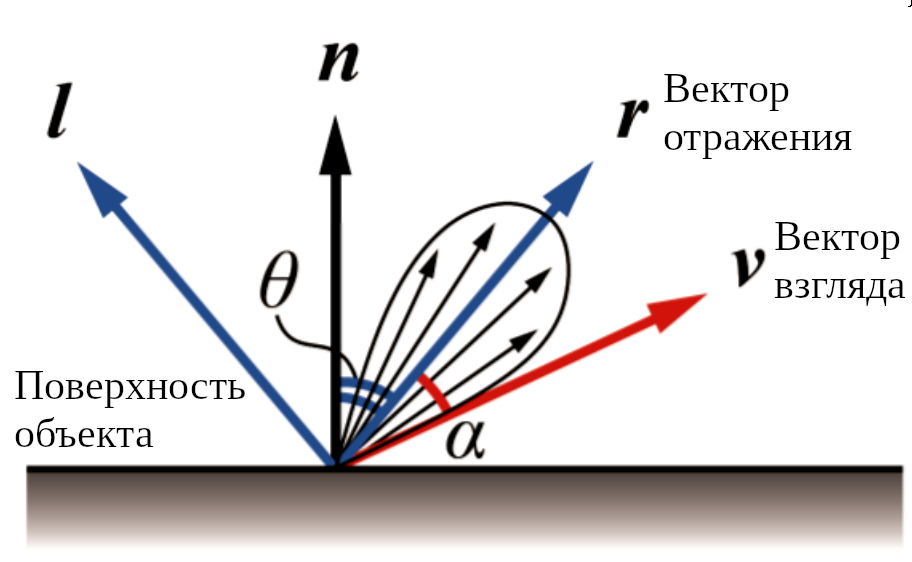
\includegraphics[width=0.66\textwidth]{img/specular_ru}
    \caption{Модель Фонга: Зеркальная составляющая света (Источник: \cite{phong})}
	\label{fig:specular}
\end{figure}

Зеркальная составляющая света, согласно \cite{phong}, рассчитывается по формуле~\ref{eq:specular}, приведённой ниже.
\begin{equation}
    I_s = k_s I_l \cos^n \alpha = k_s I_l \left| \boldsymbol{r} \cdot \boldsymbol{v} \right|^n,
    \label{eq:specular}
\end{equation}
где
\begin{itemize}
    \item $k_s$ --- коэффициент зеркального отражения,
    \item $\boldsymbol{r}$ --- вектор отражённого света,
    \item $\boldsymbol{v}$ --- вектор взгляда,
    \item $\cos \alpha$ --- угол между вектором взгляда и вектором отражённого света,
    \item $n$ --- коэффициент шероховатости поверхности.
\end{itemize}

Сумма рассеянной, фоновой и зеркальной составляющих даёт итоговый отражённый свет:
\begin{equation}
    I = k_d I_l \left| \boldsymbol{n} \cdot \boldsymbol{l} \right| + k_a I_0 + k_s I_l \left| \boldsymbol{r} \cdot \boldsymbol{v} \right|^n
    \label{eq:phong}
\end{equation}

\subsubsection{Шаги графического конвейера}

\subsection{Выбор типов и структур данных}

% \subsection{Общая архитектура разрабатываемой программы}

% Классы

\subsection*{Вывод}

% Всё, что надо планировалось, было сделано, схемы алгоритмов разработаны и т.д.
